

\tikzset{every picture/.style={line width=0.45pt}} %set default line width to 0.75pt        

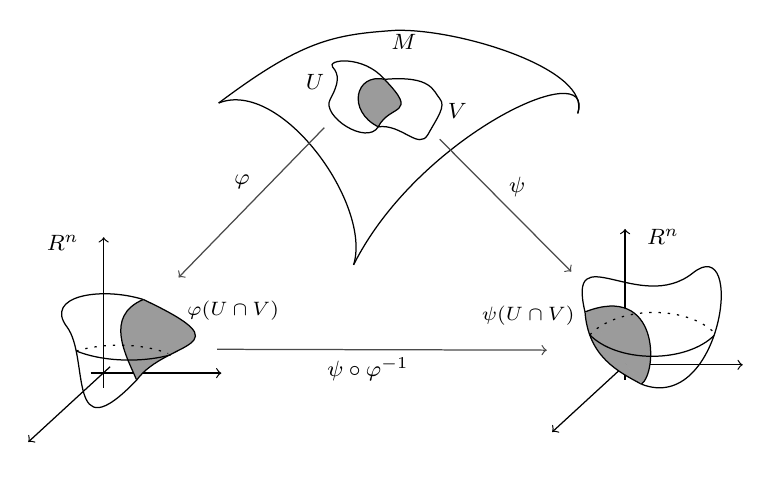
\begin{tikzpicture}[x=0.75pt,y=0.75pt,yscale=-1,xscale=1]
%uncomment if require: \path (0,300); %set diagram left start at 0, and has height of 300

%Curve Lines [id:da12253634132608959] 
\draw    (130.5,61) .. controls (160.5,49) and (204.5,110) .. (195.5,139) ;
%Curve Lines [id:da09568098876338671] 
\draw    (195.5,139) .. controls (226.5,77) and (312.5,37) .. (303.5,66) ;
%Curve Lines [id:da12952951962291093] 
\draw    (130.5,61) .. controls (170.5,31) and (185.5,28) .. (215.5,26) ;
%Curve Lines [id:da8017459310615034] 
\draw    (215.5,26) .. controls (246.5,25) and (310.5,45) .. (303.5,66) ;
%Straight Lines [id:da11165753602356343] 
\draw [color={rgb, 255:red, 74; green, 74; blue, 74 }  ,draw opacity=1, -> ]   (181.4,72.86) -- (111.19,145.03) ;
%\draw [shift={(109.8,146.46)}, rotate = 314.21000000000004] [color={rgb, 255:red, 74; green, 74; blue, 74 }  ,draw opacity=1 ][line width=0.75]    (10.93,-3.29) .. controls (6.95,-1.4) and (3.31,-0.3) .. (0,0) .. controls (3.31,0.3) and (6.95,1.4) .. (10.93,3.29) ;
%Shape: Axis 2D [id:dp8820201499438707] 
\draw[->]  (68.8,191.13) -- (131.8,191.13);
\draw[<-] (75.1,125.66) -- (75.1,198.4);
%Straight Lines [id:da7817199884965225] 
\draw[->]  (78.2,188.06) -- (38.78,224.31) ;
%\draw [shift={(37.3,225.67)}, rotate = 317.4] [color={rgb, 255:red, 0; green, 0; blue, 0 }  ][line width=0.75]    (10.93,-3.29) .. controls (6.95,-1.4) and (3.31,-0.3) .. (0,0) .. controls (3.31,0.3) and (6.95,1.4) .. (10.93,3.29)   ;
%Straight Lines [id:da21051464502306283] 
\draw [color={rgb, 255:red, 74; green, 74; blue, 74 }  ,draw opacity=1, ->]   (237,78.46) -- (300.39,142.24) ;
%\draw [shift={(301.8,143.66)}, rotate = 225.18] [color={rgb, 255:red, 74; green, 74; blue, 74 }  ,draw opacity=1 ][line width=0.75]    (10.93,-3.29) .. controls (6.95,-1.4) and (3.31,-0.3) .. (0,0) .. controls (3.31,0.3) and (6.95,1.4) .. (10.93,3.29)   ;
%Shape: Axis 2D [id:dp22295758051907422] 
\draw[->]  (320,187.13) -- (383,187.13);
\draw[<-] (326.3,121.66) -- (326.3,194.4);
%Straight Lines [id:da3563469474596257] 
\draw[->]    (330.6,183.26) -- (291.18,219.51) ;
%\draw [shift={(289.7,220.87)}, rotate = 317.4] [color={rgb, 255:red, 0; green, 0; blue, 0 }  ][line width=0.75]    (10.93,-3.29) .. controls (6.95,-1.4) and (3.31,-0.3) .. (0,0) .. controls (3.31,0.3) and (6.95,1.4) .. (10.93,3.29)   ;
%Straight Lines [id:da572071933187088] 
\draw [color={rgb, 255:red, 155; green, 155; blue, 155 }  ,draw opacity=1 ][fill={rgb, 255:red, 155; green, 155; blue, 155 }  ,fill opacity=1 ]   (94.2,155.66) -- (91,194.46) ;
%Straight Lines [id:da18438752078564646] 
\draw [color={rgb, 255:red, 155; green, 155; blue, 155 }  ,draw opacity=1 ][fill={rgb, 255:red, 155; green, 155; blue, 155 }  ,fill opacity=1 ]   (307,161.66) -- (331.8,193.66) ;
%Curve Lines [id:da951001718333709] 
\draw    (307,161.66) .. controls (298.2,124.46) and (333.4,163.26) .. (359,142.86) .. controls (384.6,122.46) and (373,211.66) .. (334.2,196.46) ;
%Curve Lines [id:da19213944484530643] 
\draw    (91,194.46) .. controls (56.6,230.46) and (68.6,183.66) .. (57.4,168.86) .. controls (46.2,154.06) and (73.4,149.26) .. (94.2,155.66) ;
%Straight Lines [id:da3787366607544964] 
\draw [color={rgb, 255:red, 74; green, 74; blue, 74 }  ,draw opacity=1, ->]   (129.8,179.66) -- (288.6,180.06) ;
%\draw [shift={(290.6,180.06)}, rotate = 180.14] [color={rgb, 255:red, 74; green, 74; blue, 74 }  ,draw opacity=1 ][line width=0.75]    (10.93,-3.29) .. controls (6.95,-1.4) and (3.31,-0.3) .. (0,0) .. controls (3.31,0.3) and (6.95,1.4) .. (10.93,3.29)   ;
%Curve Lines [id:da24270644855795598] 
\draw    (210.4,49.6) .. controls (233.4,47.66) and (233.8,55.26) .. (237,58.86) .. controls (240.2,62.46) and (235.8,68.06) .. (231.4,76.06) .. controls (227,84.06) and (218.69,70.89) .. (207.4,72.46) ;
%Curve Lines [id:da33545782983962047] 
\draw    (210.4,49.6) .. controls (200.2,37.66) and (182.2,40.06) .. (185.4,43.66) .. controls (188.6,47.26) and (188.6,51.26) .. (184.2,59.26) .. controls (179.8,67.26) and (201.8,81.66) .. (207.4,72.46) ;
%Straight Lines [id:da14052521632408] 
\draw [color={rgb, 255:red, 155; green, 155; blue, 155 }  ,draw opacity=1 ][fill={rgb, 255:red, 155; green, 155; blue, 155 }  ,fill opacity=1 ]   (210.4,49.6) -- (207.4,72.46) ;
%Curve Lines [id:da2501449241188438] 
\draw [fill={rgb, 255:red, 155; green, 155; blue, 155 }  ,fill opacity=1 ]   (207.4,72.46) .. controls (192.2,64.86) and (196.2,46.46) .. (210.4,49.6) ;
%Curve Lines [id:da2598296067011632] 
\draw [fill={rgb, 255:red, 155; green, 155; blue, 155 }  ,fill opacity=1 ]   (210.4,49.6) .. controls (227.4,67.26) and (213,61.26) .. (207.4,72.46) ;
%Curve Lines [id:da5220380098580575] 
\draw [fill={rgb, 255:red, 155; green, 155; blue, 155 }  ,fill opacity=1 ]   (91,194.46) .. controls (85.8,182.46) and (75.19,163.72) .. (94.2,155.66) ;
%Curve Lines [id:da5783963299572314] 
\draw [fill={rgb, 255:red, 155; green, 155; blue, 155 }  ,fill opacity=1 ]   (94.2,155.66) .. controls (145,179.66) and (105.4,174.86) .. (91,194.46) ;
%Shape: Arc [id:dp7983026148871659] 
\draw  [draw opacity=0] (107.37,182.33) .. controls (101.59,183.93) and (94.75,184.85) .. (87.41,184.85) .. controls (77.56,184.85) and (68.6,183.19) .. (61.92,180.47) -- (87.41,168.52) -- cycle ; \draw   (107.37,182.33) .. controls (101.59,183.93) and (94.75,184.85) .. (87.41,184.85) .. controls (77.56,184.85) and (68.6,183.19) .. (61.92,180.47) ;
%Shape: Arc [id:dp4531975717042873] 
\draw  [draw opacity=0][dash pattern={on 0.84pt off 2.51pt}] (61.92,180.47) .. controls (67.6,178.76) and (74.39,177.74) .. (81.69,177.68) .. controls (91.08,177.6) and (99.66,179.12) .. (106.14,181.69) -- (81.83,194.01) -- cycle ; \draw  [dash pattern={on 0.84pt off 2.51pt}] (61.92,180.47) .. controls (67.6,178.76) and (74.39,177.74) .. (81.69,177.68) .. controls (91.08,177.6) and (99.66,179.12) .. (106.14,181.69) ;
%Curve Lines [id:da40298571757933943] 
\draw [fill={rgb, 255:red, 155; green, 155; blue, 155 }  ,fill opacity=1 ]   (334.2,196.46) .. controls (323,190.46) and (308.6,183.26) .. (307,161.66) ;
%Curve Lines [id:da8319827009641485] 
\draw [fill={rgb, 255:red, 155; green, 155; blue, 155 }  ,fill opacity=1 ]   (307,161.66) .. controls (342.79,147.52) and (342.2,190.46) .. (334.2,196.46) ;
%Shape: Arc [id:dp5999943800568168] 
\draw  [draw opacity=0] (369.2,172.96) .. controls (363.26,178.98) and (352.14,183.03) .. (339.4,183.03) .. controls (326.46,183.03) and (315.19,178.85) .. (309.32,172.67) -- (339.4,162.9) -- cycle ; \draw   (369.2,172.96) .. controls (363.26,178.98) and (352.14,183.03) .. (339.4,183.03) .. controls (326.46,183.03) and (315.19,178.85) .. (309.32,172.67) ;
%Shape: Arc [id:dp7315027451637988] 
\draw  [draw opacity=0][dash pattern={on 0.84pt off 2.51pt}] (309.32,172.67) .. controls (315.13,166.52) and (326.15,162.21) .. (338.88,161.92) .. controls (351.82,161.63) and (363.18,165.55) .. (369.2,171.59) -- (339.34,182.05) -- cycle ; \draw  [dash pattern={on 0.84pt off 2.51pt}] (309.32,172.67) .. controls (315.13,166.52) and (326.15,162.21) .. (338.88,161.92) .. controls (351.82,161.63) and (363.18,165.55) .. (369.2,171.59) ;

% Text Node
\draw (171.2,45.8) node [anchor=north west][inner sep=0.75pt]  [font=\footnotesize]  {$U$};
% Text Node
\draw (239.6,60) node [anchor=north west][inner sep=0.75pt]  [font=\footnotesize]  {$V$};
% Text Node
\draw (136.8,94.2) node [anchor=north west][inner sep=0.75pt]  [font=\footnotesize]  {$\varphi $};
% Text Node
\draw (269.2,95.2) node [anchor=north west][inner sep=0.75pt]  [font=\footnotesize]  {$\psi $};
% Text Node
\draw (114,155.2) node [anchor=north west][inner sep=0.75pt]  [font=\scriptsize]  {$\varphi ( U\cap V)$};
% Text Node
\draw (256,157.6) node [anchor=north west][inner sep=0.75pt]  [font=\scriptsize]  {$\psi ( U\cap V)$};
% Text Node
\draw (181.6,182.4) node [anchor=north west][inner sep=0.75pt]  [font=\footnotesize]  {$\psi \circ \varphi ^{-1}$};
% Text Node
\draw (46.4,123.6) node [anchor=north west][inner sep=0.75pt]  [font=\footnotesize]  {$\mathbb{R}^{n}$};
% Text Node
\draw (335.6,120.4) node [anchor=north west][inner sep=0.75pt]  [font=\footnotesize]  {$\mathbb{R}^{n}$};
% Text Node
\draw (212.4,26.6) node [anchor=north west][inner sep=0.75pt]  [font=\footnotesize]  {$M$};


\end{tikzpicture}
